    %   Il progetto nasce dal template per il frontespizio realizzato da Marco Antonio Corallo, che ringrazio. Seguono alcuni commenti per evidenziare la presenza di alcuni pacchetti che mi sono stati utili per la stesura della tesi. Chiaramente, dipende tutto dal tipo di lavoro che uno vuole eseguire, che determina anche le diverse esigenze. Durante la stesura ho passato molto tempo su siti e forum a cercare di risolvere alcuni probelmi di formattazione, ma in generale Latex è stato piuttosto versatile. 

% Tipo di documento. L'uso di twoside implica che i capitoli inizino sempre con la prima pagina a sinistra, eventualmente lasciando una pagina vuota nel capitolo precedente. Se questa cosa è fastidiosa, è possibile rimuoverlo. 
\documentclass[a4paper, twoside,openright]{report}
\usepackage{titlesec}

% Dimensione dei margini
\usepackage[a4paper,top=2.5cm, bottom=2.5cm, left=4cm, right=2.5cm, centering]{geometry} % Default 3cm ovunque

% Interlinea
\linespread{1.5}


% Dimensione del font
\usepackage[fontsize=13pt]{scrextend} % Dipende come 12
% Lingua del testo
\usepackage[english,italian]{babel}
% Lingua per la bibliografia
\usepackage[fixlanguage]{babelbib}
\usepackage[sort&compress, numbers]{natbib}
% Codifica del testo
\usepackage[utf8]{inputenc} 
% Encoding del testo
\usepackage[T1]{fontenc}
% Permette di generare testo fittizio. Mi è stato utile 
% per capire quale sarebbe stata l'impostazione del 
% testo nella pagina prima che scrivessi un determinato paragrafo
\usepackage{lipsum}
% Per ruotare le immagini
\usepackage{rotating}
% Per modificare l'header delle pagine 
\usepackage{fancyhdr}               

% Librerie matematiche
\usepackage{amssymb}
\usepackage{amsmath}
\usepackage{amsthm}         

% Uso delle immagini
\usepackage{graphicx}
% Uso dei colori
\usepackage[dvipsnames]{xcolor}         
% Uso dei listing per il codice
\usepackage{listings}          
% Per inserire gli hyperlinks tra i vari elementi del testo 
\usepackage{hyperref}     
% Diversi tipi di sottolineature
\usepackage[normalem]{ulem}

\usepackage{algorithm2e}

% Per impostare lo spazio tra testo
\usepackage{setspace}

% -----------------------------------------------------------------

% Modifica lo stile dell'header
% \pagestyle{fancy}
% \fancyhf{}
% \lhead{\rightmark}
% \rhead{\textbf{\thepage}}
% \fancyfoot{}
% \setlength{\headheight}{12.5pt}

% Linea con intestazioni parte superiore
\pagestyle{fancy}
\fancyhf{}
\lhead{\rightmark}
\fancyfoot{}
\setlength{\headheight}{12.5pt}
 
% Stile intestazioni parte inferiore
\pagestyle{fancy}
\cfoot{\textbf{\thepage}}  % Sposta il numero di pagina in grassetto nel piè di pagina a destra
\renewcommand{\headrulewidth}{0.4pt}   % Rimuove la linea dall’intestazione
\renewcommand{\footrulewidth}{0.4pt} % Aggiunge una linea al piè di pagina
\setlength{\footskip}{25pt} % Aumenta la distanza dal contenuto per maggiore spazio, se necessario

% Rimuove il numero di pagina all'inizio dei capitoli
\fancypagestyle{plain}{
  \fancyhead{}
  \renewcommand{\headrulewidth}{0pt}
}

% Stile del codice
\lstdefinestyle{codeStyle}{
    % Colore dei commenti
    commentstyle=\color{teal},
    % Colore delle keyword
    keywordstyle=\color{Magenta},
    % Stile dei numeri di riga
    numberstyle=\tiny\color{gray},
    % Colore delle stringhe
    stringstyle=\color{violet},
    % Dimensione e stile del testo
    basicstyle=\ttfamily\footnotesize,
    % newline solo ai whitespaces
    breakatwhitespace=false,     
    % newline si/no
    breaklines=true,                 
    % Posizione della caption, top/bottom 
    captionpos=b,                    
    % Mantiene gli spazi nel codice, utile per l'indentazione
    keepspaces=true,                 
    % Dove visualizzare i numeri di linea
    numbers=left,                    
    % Distanza tra i numeri di linea
    numbersep=5pt,                  
    % Mostra gli spazi bianchi o meno
    showspaces=false,                
    % Mostra gli spazi bianchi nelle stringhe
    showstringspaces=false,
    % Mostra i tab
    showtabs=false,
    % Dimensione dei tab
    tabsize=2
} \lstset{style=codeStyle}

% Stile di codice per dimensioni maggiori, in cui ho avuto bisogno di un testo più picolo (ad esempio se si vuole inserire del codice che ha linee molto lunghe). Per usare questo stile piuttosto che il precedente, usare 

% \lstset{style=longBlock}
%  % inserire il codice...
% \lstset{style=codeStyle}

% Il secondo comando consente di tornare allo stile precedente 
\lstdefinestyle{longBlock}{
    commentstyle=\color{teal},
    keywordstyle=\color{Magenta},
    numberstyle=\tiny\color{gray},
    stringstyle=\color{violet},
    basicstyle=\ttfamily\scriptsize,
    breakatwhitespace=false,         
    breaklines=true,                 
    captionpos=b,                    
    keepspaces=true,                 
    numbers=left,                    
    numbersep=5pt,                  
    showspaces=false,                
    showstringspaces=false,
    showtabs=false,                  
    tabsize=2
} \lstset{style=codeStyle}

% Togliendo il commento al comando che segue, si inseriscono nella bibliografia anche le fonti presenti in Bibliography.bib ma non citati direttamente con il comando \cite
% \nocite{*}

% Margini prima e dopo blocchi di codice, per avere più distanza
\lstset{aboveskip=20pt,belowskip=20pt}

% Modifica dello stile dei riferimenti, con il testo in cyano
\hypersetup{
    colorlinks,
    linkcolor=CornflowerBlue,
    citecolor=CornflowerBlue
}

% Aggiunti definizioni, teoremi, linea e listing
\newtheorem{definition}{Definizione}[section]
\newtheorem{theorem}{Teorema}[section]
\providecommand*\definitionautorefname{Definizione}
\providecommand*\theoremautorefname{Teorema}
\providecommand*{\listingautorefname}{Listing}
\providecommand*\lstnumberautorefname{Linea}

\raggedbottom
%------------------------------
% Formato chapter
%------------------------------
% Stile particolare
%\usepackage[Lenny]{fncychap}
% Impostazioni per renderlo come: "1 INTRODUZIONE"
\titleformat{\chapter}[hang]
  {\normalfont\fontsize{25pt}{22pt}\bfseries} % Stile dei titoli (maiuscolo)
  {\thechapter} % Testo da visualizzare prima del numero del capitolo
  {0.5em} % Spaziatura
  %{\MakeUppercase} % Trasforma il titolo in maiuscolo
  %[]
  {}

  % Impostare spaziatura numero testo
  \titleformat{\section}{\normalfont\Large\bfseries}{\thesection}{0.5em}{}  % Per le sezioni
  \titleformat{\subsection}{\normalfont\bfseries}{\thesubsection}{0.5em}{}  % Per le sezioni


%\newcommand{\cgs}[1]{{\textcolor{brown}[\textcolor{red}{\bf{GS: }}{ \textcolor{brown}{#1]}}}}             
%\newcommand{\cmc}[1]{{\textcolor{blue}[\textcolor{magenta}{\bf{MC: }}{ \textcolor{blue}{#1]}}}}


% Impostare lo spazio a due
% \doublespacing
% Definisci i colori per il codice
\usepackage{xcolor}
\definecolor{mygreen}{rgb}{0.2588, 0.5804, 0.2471}

% Configura lo stile per il codice Python
\lstset{ 
frame=tb,                     % Aggiunge una linea sopra (t) e sotto (b)
  framesep=3pt,                 % Distanza tra il codice e la cornice
  rulesepcolor=\color{black},   % Colore della linea
  basicstyle=\ttfamily\footnotesize,      % Stile di base
  breaklines=true,                        % Spezza le righe lunghe
  commentstyle=\color{mygreen},           % Colore dei commenti
  stringstyle=\color{brown},           % Colore delle stringhe
  emph={__init__, fit, predict, detect_anomalies, decision_function,apply_kernels,generate_kernels,shape, KNN, XGBOD, apply_kernel, ROCKAD}, 
  emphstyle=\color{blue},                      % Colore per le funzioni
  language=Python                         % Linguaggio del codice
}

\usepackage{adjustbox}
\usepackage{xcolor}
\usepackage{amsmath}
% -----------------------------------------------------------------
\begin{document}
\begin{singlespace}
    % Frontespizio
\begin{titlepage}
\begin{figure}
    \centering
\includegraphics[scale=0.5]{images/Frontespizio/cherubinFrontespizio.eps}
\end{figure}

\begin{center}
    {\LARGE{ Corso di Laurea in Informatica \\}}
    \vspace{2cm}
    {\Large { TESI DI LAUREA }}\\
    \vspace{2cm}
    {\Large { Rilevamento Continuo di Anomalie nel Contesto Satellitare: una Validazione Empirica }}
\end{center}

\vspace{2cm}

\begin{minipage}[t]{0.47\textwidth}
	{\large{\bf Relatore:\\ Vincenzo Lomonaco}}
	\vspace{0.5cm}
	{\large{\bf \\Correlatore:\\ Lampei Li}}
\end{minipage}\hfill\begin{minipage}[t]{0.47\textwidth}\raggedleft
	{\large{\bf Candidato: \\ Francesco Fiaschi\\ }}
\end{minipage}

\vspace{25mm}
\hrulefill
\\\centering{\large{ANNO ACCADEMICO 2024/2025}}
\end{titlepage}
    %\begin{titlepage}
\begin{figure}[!htb]
    \centering
    
\includegraphics[keepaspectratio=true,scale=0.5]{images/Frontespizio/cherubinFrontespizio.eps}
\end{figure}

\begin{center}
    \LARGE{UNIVERSITÀ DI PISA}
    \vspace{5mm}
    \\ \large{DIPARTIMENTO DI INFORMAZIONE}
    \vspace{5mm}
    \\ \LARGE{Laurea Triennale in Informatica}
\end{center}

\vspace{12mm}
\begin{center}
    {\LARGE{\bf  Rilevamento Continuo di Anomalie nel Contesto Satellitare: una Validazione Empirica\\ \vspace{5mm}}}
    
    % Se il titolo è abbastanza corto da stare su una riga, si può usare
    
    % {\LARGE{\bf Un fantastico titolo per la mia tesi!}}
\end{center}
\vspace{30mm}

\begin{minipage}[t]{0.47\textwidth}
	{\large{Relatore:}{\normalsize\vspace{3mm}
	\bf\\ \large{Prof. Vincenzo Lomonaco} \normalsize\vspace{3mm}\bf \\ \large{Dr. Lampei Li}}}
\end{minipage}
\hfill
\begin{minipage}[t]{0.47\textwidth}\raggedleft
	{\large{Candidato:}{\normalsize\vspace{3mm} \bf\\ \large{Francesco Fiaschi}}}
\end{minipage}

\vspace{30mm}
\hrulefill
\\\centering{\large{ANNO ACCADEMICO 2024/2025}}

\end{titlepage}
    \cleardoublepage
    \title{Abstract}
\begin{abstract}
    bgnbrtgnbrtgntr
\end{abstract}

    
\tableofcontents
% Rimuovere se non si vuole la tabella delle figure
\listoffigures
\end{singlespace}

\chapter{Introduzione}
\section{Rilevamento di Anomalie nei Satelliti}
Negli anni si è fatto sempre più presente il bisogno di esplorare lo spazio puntando sempre più lontano, studiando e comprendendo le regole e le strutture dell'universo partendo dall'osservazione di quest'ultimo. Con l'avanzare della tecnologia abbiamo potuto avvicinarci allo spazio tramite i satelliti posizionati in orbita intorno alla Terra; questi sono circa 3500 attivi e si è fatta sempre più importante la richiesta di rilevare le anomalie di tali satelliti e comunicandole alla stazione di controllo, portando un aumento nello scambio di informazioni con un costo non irrilevante data la banda limitata.
Prima dell'avvento dell'intelligenza artificiale la rilevazione delle anomalie era lasciata a un'analisi statica delle componenti, controllo di qualità con regole e soglie fisse, questo ovviamente portava ad avere un'alta probabilità di ricevere tante segnalazioni di anomalie non rilevanti o date da cambiamenti nei riferimenti che creano un diverso ambiente vanificando i controlli statici.
Con l'intelligenza artificiale siamo riusciti ad avere un rilevamento adattivo in base all'ambiente che portava ad avere meno false anomalie ma anche questo approccio portava con se delle problematiche: l'algoritmo di intelligenza artificiale veniva allenato nel centro di controllo su dati reali e poi spedito sul satellite, ogni volta che bisognava cambiare i parametri dell'algoritmo bisognava ripetere tutto il processo dato che i satelliti all'interno hanno un processore molto poco prestante e quindi non sufficiente ad eseguire l'allenamento degli algoritmi, sprecando così tanta banda e molto tempo di trasmissione.

\section{NASA ed ESA}
Negli anni sia la NASA (National Aeronautics and Space Administration) che l'ESA (Agenzia Spaziale Europea) hanno pubblicato molteplici dataset contenenti dati reali di missioni e relativi benchmark sull'esecuzione di algoritmi di intelligenza artificiale per trovare il giusto compromesso tra efficacia e efficienza di un algoritmo, focalizzandosi maggiormente sul trovare l'algoritmo migliore per il rilevamento delle anomalie.

I dataset sono stati resi pubblici per incentivare la comunità a contribuire alla ricerca di nuove tecniche di monitoraggio e rilevamento delle anomalie, potendo usare dati reali.

\section{Obbiettivo}
Partendo dai dati proposti nel più semplice dataset OPS-SAT e successivamente comprendendo il benchmark di NASA, vogliamo analizzare quali test sono stati effettuati per capire come poter fare un ulteriore passo in avanti nel rilevamento continuo di anomalie, cercando di rendere più efficiente un algoritmo già efficace, in modo da poterlo allenare direttamente sul satellite, limitando così lo scambio di comunicazioni e restringendo ancora di più il rilevamento di false anomalie.

Tutto questo processo è dedito a trovare un algoritmo che abbia un giusto compromesso tra efficienza ed efficacia, così che possa rilevare in modo corretto la maggioranza delle anomalie senza però avere un costo molto alto in termini di consumo di banda e di risorse del satellite.

In primo luogo procederemo a scendere più nello specifico aggiungendo o aggiustando i parametri di alcuni algoritmi tra cui XGBOD.
Per validare l'implementazione fatta portiamo a sostegno risultati ottenuti effettuando test e confronti tra un'implementazione standard e la nostra proposta mettendo a paragone le metriche di valutazione.

In secondo luogo vogliamo proporre un'implementazione di due algoritmi, ROCKET e ROCKAD, sui quali sono stati pubblicati articoli recentemente dove si afferma la loro bassa complessità e le ottime performance nelle timeseries.
Per questi motivi abbiamo adattato questi algoritmi per il rilevamento delle anomalie su timeseries, applicando preprocessing ai dati estratti dai dataset. Partendo dal dataset OPS-SAT tramite vari test abbiamo estrapolato vari risultati di test e metriche corrispondenti, per poi spostarci su NASA, al quale accediamo tramite SpaceAI $^{\cite{SpaceAI}}$ riportando anche qui metriche di valutazione allo scopo di poter confrontare gli algoritmi in termini di efficacia.

\chapter{Aquisizione dei Dati}
Procediamo ora a descrivere i dataset contenenti dati di telemetrie registrati negli anni e resi pubblici in modo da poter sperimentare e migliorare gli algoritmi già presenti.

\section{Dataset ESA}

Il dataset di riferimento più importante per la rilevazione delle anomalie è quello fornito dall'ESA (European Space Agency) che conta dati di tre missioni. Di queste solo i dati di due vengono utilizzati per creare il benchmark, per le caratteristiche dell'insieme di dati; infatti in \textit{"Mission 3"} abbiamo: poche anomalie e per lo più banali, un gran numero di buchi di comunicazione e segmenti non validi.

Nell'articolo in questione i dati satellitari grezzi di \textit{"Mission 1"} e \textit{"Mission 2"} vengono preprocessati per renderli uniformi e quindi utilizzabili con la maggior parte degli algoritmi.

In questa fase utilizziamo OXI$^{\cite{OXI_annotation_tool}}$ per l'etichettatura collaborativa dei dati da cui si è potuto estrarre delle telemetrie che rappresentano periodi di funzionamento nominale e anomalo. Tutti i dati sono stati sottoposti ad una doppia fase di etichettatura e controllo.

I canali sono divisi tra "target" e "non target" dove quest'ultimi sono usati per gli algoritmi solo come informazioni addizionali. Un canale target, quello usato per rilevare le anomalie, è diviso in gruppi di dati con caratteristiche simili così da rendere più facile per l'algoritmo processarli ed interpretarli e, nel caso, allenarlo solo sul quel gruppo specifico.
\pagebreak

\begin{table}[h]
    \centering
    \begin{tabular}{|l|c|c|}
        \hline
         \textbf{}& \textbf{Mission 1} & \textbf{Mission 2}\\
         \hline
        \textbf{Channels} & 76 & 100\\
        Target/Non target & 58/18 & 47/53\\
        \hline
        \textbf{Telecommands} & 698 & 123\\
        \hline
        \textbf{Annotate Events} & 200 & 644 \\
        Anomalies& 118 & 31\\
        Rare Nominal Events &78  & 613\\
        Univariate/Multivariate& 32/164 & 9/635\\
        \hline
    \end{tabular}
    \caption{Configurazione Dataset ESA}
    \label{tab:costituzioneESA_dataset}
\end{table}

Possiamo osservare dalla Tabella \ref{tab:costituzioneESA_dataset} che la densità di anomalie in termini di punti di dati annotati, varia tra $0,57\%$ per la \textit{"Mission 2"} e $1,80\%$ per la \textit{"Mission 1"} questo va a confermare un'impronta più realistica rispetto ai dataset meno recenti che avevano una densità di anomalie estremamente più alta ed irrealistica.

\section{Motivazioni}
Il dataset ESA pecedentemente descritto porta alla risoluzione di vari problemi noti nell'ambito della rilevazione di anomalie.
Il primo problema come si evidenzia nei dataset \textit{NASA Soil Moisture Active Passive} (SMAP) e  \textit{Mars Science Laboratory} (MSL) i quali offrono brevi frammenti di segnali e comandi correlati da 55 e 27 parametri di telemetria, rispettivamente, con un totale di 105 anomalie annotate; infatti abbiamo una densità di anomalie irrealistica, alto numero di anomalie banali, verità di bse etichettate in maniera errate e una mancanza di corrlazione tra comandi e canali. Quindi è stato deciso che questi dataset non andrebbero usati per il benchamrking del rilevamento delle anomalie.
Il senondo problema invece rappresenta la mancanza di annotazione di eventi anomali, alcuni esempi sono gli insiemi di dati di \textit{Mars Express6} e \textit{NASA WebTCAD7}.

Il dataset ESA risolve i problemi elencati ma nasce come dataset di missioni su larga scala, le quali sono molto complesse e stabili portando con se problemi non più relativi alla distribuzione delle anomalie ma improntati verso problemi di esecuzione e potenza di calcolo.

Il dataset che intrudurremo dopo è concettualmente diverso, infatti affronta una missione ESA OP-SAT molto semplificata al fine di rendere più accessibile l'uso, oltre ad essere di dimensione considerevolmente minore.

Questo processo di apertura è reso anche tramite la sostituzione giornaliera dell'intero sistema software fino al sistema operativo del satellite così da consentire alle persone che sperimentano di caricare il proprio software a bordo e a terra. Per implementare questa funzionalità venne usato FDIR$^{\cite{FDIR}}$

Le telemetrie grezze sono caratterizzate da molte lacune nei dati ed altre imprecisioni, queste vengono curate da ingegneri ed esperti nei modelli di apprendimento automatico per rendere l'insieme di dati fruibile alla creazione di tecniche di rilevamento delle anomalie basate sui dati.
Una di queste modifiche è la seguente:

\begin{quote}
    Selezione e annotazione di verità di base (ground-truth) di 2123 brevi frammenti di telemetria a canale singolo ossia serie temporali univariate$^{\cite{10.1007/978-3-031-35995-8_21}}$, registrate in 9 canali di telemetria.
\end{quote}

Infine questo dataset con il relativo benchmark e tutti i dati al suo interno disponibili è stato messo a disposizione per aiutare la comunità nella ricerca di nuovi approcci per la rilevazione delle anomalie, confrontandosi tra di loro in modo imparziale ed equo così da affrontare anche il problema della riproducibilità nell'ambiente dell'apprendimento automatico (dato che i dataset sono sono uniformati, l'ambiente di esecuzione diverso e varie metriche usate) 

Tutto ciò che è stato sviluppato con l'aiuto di questo dataset verrà convalidato con il lancio alla fine del 2025 del satellite successore OP-SAT VOLT (dopo averli distribuiti a bordo del satellite).


\section{OP-SAT Dataset}
Nel dataset OP-SAT sono contenuti i dati delle telemetrie del satellite OP-SAT dell'ESA (Figura \ref{fig:OP-SAT_satellite}). Questo satellite di tipo CubeSat aveva dimensione 3 unità (3U dove 1U=10cm$^3$), esso ormai non è più in orbita, era stato lanciato a Dicembre del 2019 con lo scopo di dimostrare l'elaborazione dei dati in orbita e di generare dati utili come immagini satellitari e telemetrie.

\begin{figure}[h]
    \centering
    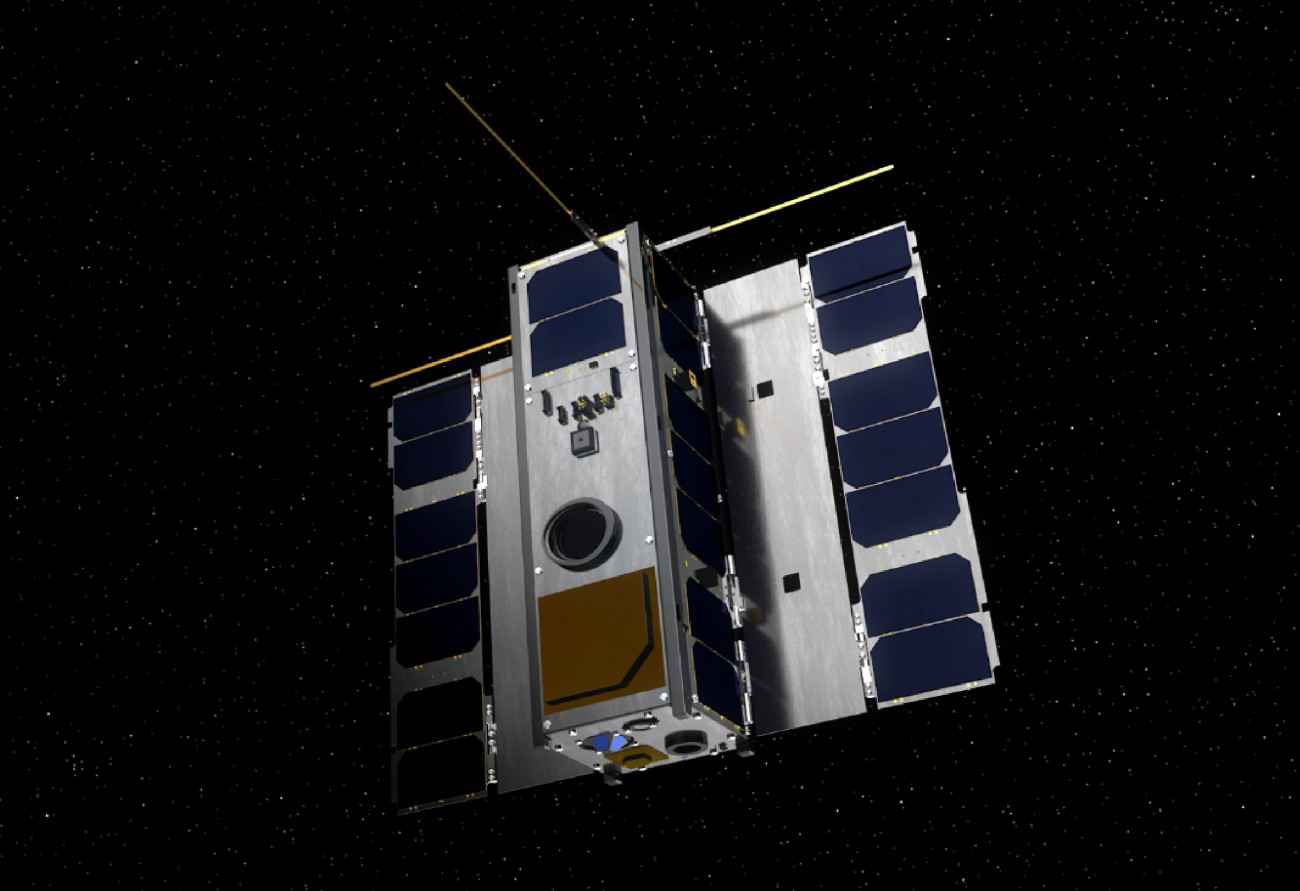
\includegraphics[width=0.5\linewidth]{images/Capitolo2/OP-SAT_satellite.png}
    \caption{Satellite OP-SAT. Fonte: Eropean Space Agency}
    \label{fig:OP-SAT_satellite}
\end{figure}

Come nel dataset precedente anche qui i dati hanno bisogno di essere preprocessati per renderli fruibili alla maggior parte degli algoritmi (OXI$^{\cite{OXI_annotation_tool}}$). In questo caso sono state progettate 18 caratteristiche per l'attività di rilevamento delle anomalie, ossia sono stati estratti tratti significativi dai dati. Questo processo è chiamato Feature Extraction e serve per ridurre la complessità dei dati in ingresso rendendoli più significativi.

Tutti i segmenti ricavati rappresentano le sfide che dobbiamo affrontare con i dati delle telemetrie, ognuno di questi è composto da:
\begin{itemize}
    \item $\langle$\texttt{timestamp}$\rangle$: rappresenta il marcatore temporale nel momento della registrazione;
    \item $\langle$\texttt{channel}$\rangle$: è il nome del canale;
    \item $\langle$\texttt{value}$\rangle$: è il valore del segnale acquisito;
    \item $\langle$\texttt{label}$\rangle$: rappresentano le annotazioni certe, quelle annotate manualmente;
    \item $\langle$\texttt{segment}$\rangle$: rappresenta il numero consecutivo del segmento;
    \item $\langle$\texttt{sampling}$\rangle$: tasso di campionamento;
    \item $\langle$\texttt{train}$\rangle$: che indica se il segmento appartiene al training set.
    
\end{itemize}

Il dataset è stato diviso in una parte di allenamento, Training Set ($T$), ed una di test, Test Set ($\Psi$). Questi rappresentano rispettivamente i dati usati per l'allenamento del modello e i dati usati per fare le valutazioni delle performance dell'algoritmo.

\begin{table}[h]
    \centering
    \begin{tabular}{|l|c|c|c|}
        \hline
        \textbf{Classi} &\textbf{Training Set} ($T$) & \textbf{Test Set ($\Psi$)}&\textbf{Total} \\
        \hline
         Nominali& 1273&416 &1689 \\
         Anomalie& 321&529 &434\\
         \hline
    \end{tabular}
    \caption{Composizione Dataset OP-SAT}
    \label{tab:dataset_op-sat}
\end{table}

Le classi, nominali e anomalie, rappresentano rispettivamente segmenti che rispettano valori normali o attesi e segmenti invece che superano questi valori o discordano dai valori attesi.
Partendo dai benchmark effettuati su questi due dataset, analizzeremo le metriche e le prestazioni utilizzando in modo più specifico il secondo dataset (OP-SAT) che contiene dati più rilevanti per il nostro obbiettivo.


\chapter{Misure di Valutazione}
Analizzeremo ora le misure che ci permettono di valutare le prestazioni di un modello allenato sui dati del training set, quindi con i relativi pesi calcolati. I modelli vengono provati sul test set ed otteniamo le seguenti metriche:
\begin{itemize}
    \item \textbf{Accuratezza}: rappresenta la percentuale di previsioni corrette (TP - True Positive) su tutti i casi possibili, tiene in considerazione anche i veri negativi (TN).
    Questa misura ci indica quanto ci stiamo avvicinando ai dati di allenamento.
    
    \textit{Formula:}
        \begin{equation}
            \frac{TP+TN}{TP+TN+FP+FN}
        \end{equation}
    
    \item \textbf{Precisione}: rappresenta la percentuale di anomalie vere rilevate in confronto a tutte le anomalie segnalate quindi la percentuale di veri positivi.

    \textit{Formula:}
        \begin{equation}
            \frac{TP}{TP+FP}
        \end{equation}
    Nel nostro caso questa metrica è particolarmente importante dati che un valore troppo basso significherebbe un alta probabilità di avere falsi positivi portando quindi uno spreco di banda ed energia per mandare i messaggi ed un allarme che richiede un intervento non necessario.

    \item \textbf{Richiamo}: rappresenta la percentuale di rilevare tutte le anomalie vere tenendo quindi in considerazione anche le anomalie non rilevate (FN). Questa misura è anche detta sensibilità.

    \textit{Formula:} 
    \begin{equation}
        \frac{TP}{TP+FN}
    \end{equation}
    Nel contesto dei satelliti questa metrica è cruciale dato che con un valore basso avremmo un grande numero di falsi negativi (FN) che quindi senza intervento potrebbero portare a conseguenze molto gravi.
    
    \item \textbf{$F_1$ score}: rappresenta una media armonica tra precisione e recupero dove il massimo si ottiene con il valore uno e il minimo a zero.

    \textit{Formula:}
    \begin{equation}
        F_1=\frac{2*TP}{2*TP+FP+FN}
    \end{equation}
    Questa misura nel nostro caso che cerchiamo un buon compromesso tra precisione e richiamo per non avere un alto numero né di falsi negativi né di falsi positivi. Questo porta ad un equilibrio tra precisione e capacità di rilevazione.

    \item \textbf{Coefficiente di correlazione di Matthews (MCC)}$^\cite{matthew}$: rappresenta una misura della qualità del modello con dati molto variabili.

    \textit{Formula:}
    \begin{equation}
        \frac{TP\cdot TN-FP\cdot FN}{\sqrt{(TP+FP)\cdot (TP+FN)\cdot(TN+TP)\cdot(TN+FN)}}    
    \end{equation}
    Questa misura è particolarmente indicata per il rilevamento delle anomalie dato che concede la stessa importanza a veri positivi, falsi positivi, veri negativi e falsi negativi.

    \item \textbf{L'area sotto la curva ROC (AUC$_\text{ROC}$}$^\cite{ROC_google}$$^\cite{ROC}$): rappresenta il rapporto tra il tasso di veri positivi e il tasso di falsi positivi (Figura: \ref{fig:Curva ROC})
    \begin{figure}
        \centering
        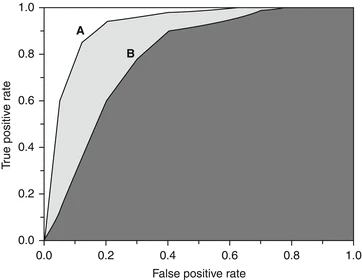
\includegraphics[width=0.5\linewidth]{images//Capitolo3/Curva ROC.png}
        \caption{Curva ROC}
        \label{fig:Curva ROC}
    \end{figure}
    Permette di osservare come varia il richiamo in funzione della metrica di precisione. Può anche essere usato per scegliere il modello migliore tra due guardando semplicemente l'area sotto al grafico, quella con l'area più grande è generalmente quello migliore.
    
    \item \textbf{Area sotto la curva Precisione-Richiamo (AUC-PR)}: rappresenta un semplici modo per sintetizzare le prestazioni generali di un modello, più alto è il valore più avrà un numero di predizioni alto. Non vengono considerati i veri positivi nella curva precisione-richiamo.
\end{itemize}
In queste formule per il calcolo delle metrica abbiamo usato TP per rappresentare i veri positivi ossia i segmenti delle telemetrie correttamente identificati come anomalie, TN per i veri negativi cioè segmenti correttamente identificati come nominali ossia regolari), FP per i falsi positivi ossia i segmenti erratamente classificati anomalie e FN per i falsi negativi che rappresentano i segmenti erratamente classificati come non anomalie.
Tutte le metriche descritte possono assumere valori tra $[0,1]$ tranne MCC che assume valori tra $[-1,1]$.
Tutte le metriche però più si avvicinano ad uno e più il modello testato risulta migliore rispetto ad uno con valori inferiori delle stesse.

Le metriche viste precedentemente ci serviranno successivamente per valutare come poter migliorare in termini di efficienza mantenendo livelli buoni delle metriche fondamentali per il rilevamento delle anomalie, non andando ad intaccare il funzionamento degli algoritmi.

\chapter{Valutazione Modelli}
In questo capitolo andremo ad analizzare gli algoritmi di nostro interesse, ossia XGBOD, ROCKED e ROCKAD.
Questi algoritmi lavorano con le timeseries, le quali sono una sequenza di dati registrati ad intervalli di tempo consecutivi. Ogni punto della serie è associato ad un timestamp il quale indica il momento in cui è stato registrato.

\section{XGBOD}
XGBOD (eXtreme Gradient Boosting for Outlier Detection) è una struttura composta in tre fasi:
\begin{enumerate}
    \item Genera nuove rappresentazioni di dati: vengono applicati vari metodi di rilevamento di anomalie non supervisionati ai dati originali per ottenere punteggi di anomalie, questi rappresentano la nuova vista dei dati;
    \item Seleziona i punteggi rilevanti: i punteggi ottenuti nella fase precedente vengono filtrati per usare sollo quelli utili, quest'ultimi sono combinati combinati con le caratteristiche iniziali creando un nuovo spazio delle caratteristiche arricchito;
    \item Addestramento del modello XGBoost: viene addestrato il modello XGBoost su questo nuovo spazio delle caratteristiche e le previsioni determinano se ogni dato è un'anomalia o no.
\end{enumerate}
Utilizziamo XGBOD invece che XGBoost direttamente perché quest'ultimo essendo un modello supervisionato ha bisogno di dati etichettati e soprattutto con anomalie rare, non facili da etichettare, XGBOD aggiunge una parte di preprocessing che aggiunge informazioni al set di dati con punteggi di anomalie.
XGBOD utilizza metodi di rilevamento non supervisionato come Isolation Forest, Local Outlier Factor, ecc..

\subsection{XGBoost}
Il modello XGBoost di tipo supervisionato, si sviluppa con un processo iterativo di addestramento di alberi decisionali deboli (alberi decisionali poco profondi e quindi poco accurati), questi vengono combinati tra di loro portando un miglioramento progressivo delle prestazioni del modello.

XGBoost è composto da pochi passi ma ripetuti iterativamente: come primo passo vengono calcolati i residui, la differenza tra le previsioni iniziali e i valori reali; questi sono i valori che vogliamo ridurre. Con questi valori il modello addestra un insieme di alberi decisionali deboli, dove ognuno cerca di correggere questi valori migliorando le previsioni del modello precedente. Tutti gli alberi vengono aggiunti al modello complessivo di XGBoost, che aggiorna le sue previsioni combinando tutti gli alberi precedentemente costruiti.

Per regolare tutto questo processo sono applicate internamente tecniche di limitazione e regolazione per evitare un overfitting del modello. All'interno di XGBoost è presente anche una metrica chiamata \textit{tasso di apprendimento} che permette di decidere quanto un albero incide sul risultato finale minimizzando così gli errori di percorso.

\subsection{Risultati ottenuti}
Qui sono elencati i risultati ottenuti effettuando varie prove con parametri diversi per ottimizzare XGBOD ed ottenere il miglior compromesso tra efficienza ed efficacia.
\pagebreak
\begin{table}[h]
    \centering
    \begin{adjustbox}{max width=\textwidth}
        \begin{tabular}{|c|c|c|c|c|c|c|c|c|}
        \hline
        \textbf{Modello} & \textbf{Accuracy} &\textbf{Prec.}  & \textbf{Recall} & \textbf{F1} & \textbf{MCC} & \textbf{auc-pr} & \textbf{auc-roc} & \textbf{Nscore}\\
     \hline
            \textbf{M+P} & 0.97 & 0.945 & 0.912 &0.928  & 0.909 & 0.973 & 0.992 &0.92 \\
            \hline
             \textbf{Early}& 0.97 & 0.971 & 0.885 & 0.926 & 0.909 & 0.969 & 0.99 & 0.912 \\
             \hline
             \textbf{+M}& 0.968 & 0.944 & 0.903 & 0.923 & 0.903 & 0.974 & 0.91 & 0.92 \\
             \hline
             \textbf{P}& 0.964 & 0.943 & 0.885 & 0.913 & 0.891 & 0.972 & 0.991 & 0.912 \\
             \hline
             \textbf{Senza P}& 0.962 & 0.935 & 0.885 & 0.909 & 0.886 & 0.977 & 0.992 & 0.912 \\
             \hline
             \textbf{Grid}& 0.947 & 0.989 & 0.761 & 0.86 & 0.839 & 0.898 & 0.945 & 0.969 \\
             \hline
        \end{tabular}
    \end{adjustbox}
    \label{tab:XGBOD_table}
    \caption{Prove esecuzione di XGBOD}
\end{table}

LEGENDA:
\begin{itemize}
    \item M+P: significa più modelli e parametri
    \item Grid: gridsearch con modelli
    \item EarlyStop: ossia viene utilizzato un meccanismo di EarlyStop che ferma l'esecuzione dell'algoritmo quando gli iperparametri non migliorano più per una numero definito di cicli.
\end{itemize}

Dalla Tabella \ref{tab:XGBOD_table} possiamo vedere che il miglior risultato è quello che utilizza più modelli per l'addestramento e i parametri modificati al fine di efficientare l'esecuzione. Oltre ad avere dei risultati ottimi l'esecuzione rimane praticamente istantanea sul nostro dataset di esempio OPS-SAT.

\section{Rocket}
Rocket è un algoritmo convoluzionale o anche detti reti neurali convoluzionali (CNN), lavorano su dati con una struttura a griglia come immagini e serie temporali e sono progettati per riconoscere pattern all'interno dei dati tramite operazioni di convoluzione.
Vengono utilizzati i kernel\footnote{Matrice di pesi usata per eseguire operazioni di filtraggio per estrarre caratteristiche specifiche, opera tramite moltiplicazioni}, che operando sui dati in input estraggono caratteristiche locali dei dati (features), in questa fase possono essere applicate tecniche di centratura, ovvero aggiungere dei bordi attorno all'input così da mantenere le dimensioni dopo aver applicato il kernel, questo di chiama padding.

Ci sono tecniche applicabile a rocket come il pooling che ha lo scopo di ridurre la dimensione e quindi a rendere l'algoritmo meno sensibile alle traslazioni, vediamo due tecniche:
\begin{itemize}
    \item Max Pooling: prende solo il valore massimo in una finestra specifica riducendo la dimensione dell'input
    \item Avarege Pooling: riduce la dimensione prendendo la media dei valori in una finestra
\end{itemize}

Il passaggio finale è il passaggio per gli strati; i dati vengono appiattiti (flattering) fatti passare attraverso uno o più strati completamente connessi per la classificazione o la regressione, per ottenere il risultato desiderato.

Rocket in particolare utilizza i kernel convoluzionali casuali, generandone un gran numero di questi con parametri scelti casualmente, come lunghezza del kernel e pesi.
Questi kernel filtrano i dati delle serie temporali producendo una serie di features; utilizzando tecniche di pooling viste in precedenza otteniamo statistiche riassuntive da queste features.
Questa procedura viene ripetuta per tutti i kernel portando ad un enorme quantità di caratteristiche e quindi una maggiore possibilità di estrarre tutti i pattern comuni.

Le caratteristiche estratte vengono poi date in input ad algoritmi di classificazione, tipicamente una regressione logistica data la sua scalabilità e velocità su grandi dataset, esso viene addestrato su queste caratteristiche per effettuare la classificazione delle serie temporali.

\subsection{Implementazione}
Per implementare Rocket abbiamo usato le funzioni che il relativo paper$^{\cite{paper_rocket}}$ ci aveva fornito:
\begin{lstlisting}[language=Python]
def generate_kernels(input_length, num_kernels)
def apply_kernel(X,weights, length, bias, dilation, padding)
def apply_kernels(X, kernels)
\end{lstlisting}
I parametri più importanti sono:
\begin{itemize}
    \item Numero di kernel (num-kernels): rappresenta il numero di kernel casuali da generare, il valore predefinito è 10000, un numero maggiore di kernel tende a migliorare l'accuratezza della classificazione ma di conseguenza aumenta la complessità e quindi il tempo di calcolo;
    \item Lunghezza del kernel (input-length): rappresenta la lunghezza del singolo kernel, questa è casuale e determina quanto della serie temporale viene considerato durante la convoluzione;
    \item Dilatazione: è un parametro che controlla la distanza tra i punti analizzati nel kernel, rocket usa varie dilatazioni per catturare caratteristiche a diverse scale temporali;
    \item Padding: determina come vengono gestiti i bordi delle serie temporali durante la fase di convoluzione;
\end{itemize} 

I vantaggi di ROCKET sono:
\begin{itemize}
    \item Efficienza computazionale elevata: è progettato per essere estremamente veloce e scalabile in modo che possa gestire grandi dataset in tempi ristretti;
    \item Robustezza: dato che si basa su kernel casuali consente di generalizzare bene su nuovi problemi senza la necessità di mettere appunto gli iperparametri;
    Semplicità: rocket permette di usare un solo iperparametro ossia il numero di kernel, riducendo così la complessità associata al perfezionamento rispetto ad altri metodi di classificazione delle serie temporali.
\end{itemize}
Come primo aspetto abbiamo eseguito in locale gli esperimenti del paper di rocket per avere una validazione empirica dell'algoritmo ottenendo gli stessi risultati della tabella del paper$^{\cite{paper_rocket}}$, successivamente ho provato l'implementazione proposta da me sui medesimi dataset ottenendo i risultati della Tabella \ref{tab:Rocket_paper}.
\begin{table}[h!]
    \centering
    \begin{adjustbox}{max width=\textwidth}
        \begin{tabular}{|c|c|c|c|c|c|c|c|}
        \hline
             \textbf{Dataset} & \textbf{Accuracy} &\textbf{Precision}  & \textbf{Recall} & \textbf{F1} & \textbf{MCC} & \textbf{auc-pr} & \textbf{auc-roc}\\
            \hline
            Coffee &1.0&1.0 & 1.0& 1.0& 1.0& 1.0& 1.0\\
             \hline
             Computers& 0.704& 0.713& 0.704& 0.701& 0.417& 0.358& 0.753\\
             \hline
             Adiac&0.777 &0.823 &0.777 &0.761 & 0.773& 0.79& 0.978\\
             \hline
             ArrowHead&0.771 &0.809 &0.771 &0.756 &0.69 &0.88 &0.942 \\
             \hline
             BeetleFly&0.85 &0.885 &0.85 &0.847 &0.834 &0.331 &1.0 \\
             \hline
             CinCECGTorso& 0.823& 0.831& 0.823& 0.822& 0.767& 0.914& 0.963\\
             \hline
             CBF& 0.992& 0.992& 0.992& 0.992&0.988 &1.0 &1.0 \\
             \hline
             ChConcentration&0.782 &0.778 &0.782 &0.774 &0.633 &0.813 &0.902 \\
             \hline
             GunPoint&1.0 &1.0 &1.0 &1.0 &1.0 & 0.315&1.0 \\
             \hline
             Ham&0.657 &0.658 &0.657 &0.655 &0.314 &0.37 &0.734 \\
             \hline
             HandOutlines&0.916 &0.917 & 0.916&0.915 & 0.817&0.963 &0.96 \\
             \hline
             InlineSkate&0.705 &0.708 & 0.705&0.7 & 0.404&0.865 &0.838 \\
             \hline
             Lightning2&0.738 &0.743 & 0.738&0.733 & 0.473&0.829 &0.805 \\
             \hline
             Mallat&0.943 &0.951 & 0.943&0.944 & 0.936&0.977 &0.994 \\
             \hline
             PhalanxTW& 0.552 &0.516 & 0.552&0.523 & 0.419&0.438 &0.822 \\
             \hline
        \end{tabular}
    \end{adjustbox}
    \label{tab:Rocket_paper}
    \caption{Esecuzione di rocket su dataset "BakeOff"}
\end{table}
\pagebrake
Nei risultati che osserveremo successivamente nella Tabella \ref{tab:RocketOPS_SAT}, sono state effettuate molte prove con varie modalità, una unsepervised quindi usando rocket per estrarre una grande quantità di caratteristiche e tramite una treshold fare la classificazione senza aver effettuato un training con le etichette dei risultati.
Una treshold è una soglia, che indica il valore di riferimento per decidere quando una predizione deve essere classificata come positiva  o negativa, in questo caso quando un valore deve essere considerato o no anomalo.
La seconda modalità che abbiamo osservato è supervised effettuando quindi il training sulle features trovate da rocket passando però le etichette delle classificazioni. Per questo abbiamo utilizzato vari algoritmi supervised pe vedere le varie performance e trovare il migliore.
Abbiamo anche osservato una modalità ibrida, ossia al posto di utilizzare una treshold o un algoritmo supervised abbiamo puntato su uno unsupervised (KNN) facendo il trining sulle feaures e restituendo delle prediction e delle classificazioni.

\texttt{RidgeClassifierCV}: è il modello usato nella demo del paper di rocket ed ho riscontrato metriche migliori anche nei nostri test.
\begin{table}[h]
    \centering
    \begin{tabular}{|c|c|c|c|c|c|c|c|c|}
    \hline
 \textbf{Modalità} & \textbf{Acc.} &\textbf{Prec.}  & \textbf{Recall} & \textbf{F1} & \textbf{MCC} & \textbf{auc-pr} & \textbf{auc-roc} & \textbf{NScore}\\
 \hline
        \multicolumn{9}{|c|}{\textbf{Unsupervised}} \\
        \hline
        \textbf{Treshold} & 0.834 & 0.963 & 0.23 &0.371  & 0.424 & 0.726& 0.772 &0.646 \\
        \hline
        \multicolumn{9}{|c|}{\textbf{Supervised}} \\
        \hline
         \textbf{RidgeCV} & 0.977 & 0.972 & 0.92 &0.945  & 0.932 & 0.962& 0.984 &0.929 \\
        \hline
        \textbf{LogisticReg} & 0.974 & 0.963 & 0.912 &0.936  & 0.92 & 0.964& 0.986 &0.92 \\
        \hline
        \textbf{RidgeReg} & 0.864 & 0.936 & 0.389 &0.55  & 0.554 & 0.871& 0.94 &0.92 \\
        \hline
        \multicolumn{9}{|c|}{\textbf{Ibrid Unsupervised}} \\
        \hline
        \textbf{KNN} & 0.834 & 0.963 & 0.23 &0.371  & 0.424 & 0.726& 0.772 &0.646 \\
        \hline
    \end{tabular}
    \label{tab:RocketOPS_SAT}
    \caption{Algoritmi eseguiti su OPS-SAT}
\end{table}

\pagebreak
Riportiamo qui il codice dell'implementazione degli algoritmi più importanti:
il primo rappresenta rocket con la treshold come decision function:
\lstinputlisting{listings/Capitolo4/RocketTreshold.py}
La seconda implementazione è quella relativa a rocket con RidgeClassifierCV:
\lstinputlisting{listings/Capitolo4/RocketRidgeClassifierCV.py}

\section{Rockad}


%\include{chapters/Capitolo5}
\chapter{Panoramica sull'Efficientamento}
Efficientare un algoritmo significa renderlo eseguibile in maniera ottimizzata anche con macchine con caratteristiche molto restringenti, come nel caso dei satelliti, con poche risorse hardware come ad esempio la CPU poco performante.
Nel nostro caso effettuiamo un Transfer Learning, ossia il riuso di un modello già addestrato su un dataset, riadattandolo al nuovo compito o dataset che vogliamo utilizzare. Questo processo può essere effettuato in diversi modi:
\begin{itemize}
    \item Estrazione delle Caratteristiche: consiste nell'estrarre caratteristiche utili dai dati senza modificare i pesi calcolati nel training precedente;
    \item Fine-Tuning:
    \begin{itemize}
        \item Addestramento sull'intera rete: in questo caso aggiorniamo i pesi eseguendo di nuovo il training sul nuovo dataset;
        \item Addestramento del Classificatore Finale: aggiorniamo solo gli stati più profondi (finali) della rete mentre i pesi dei primi rimangono congelati;
        \item Addestramento a Blocchi: i pesi dei blocchi vengono aggiornati singolarmente effettuando l'addestramento blocco per blocco.
    \end{itemize}   
\end{itemize}

Per il nostro scopo possiamo effettuare diversi tipi di fine-tuning:
\begin{enumerate}
    \item Precisione dei Pesi: i pesi derivati dall'addestramento della rete hanno una precisione, ossia il numero di bit che vengono usati per rappresentare il numero, diminuendola impiegheremo meno memoria necessaria e velocizzeremo la velocità di calcolo;
    \item Riducendo la Complessità del Modello: possiamo eliminare nodi poco significativi tramite la tecnica detta pruning, diminuendo anche la quantità di operazioni necessarie;
    \item Compromesso Concorrenza Aggiornamento pesi: il batch size ossia il numero di pesi che si attende prima di aggiornarli evitando di farlo ogni volta per non sprecare risorse di calcolo, incentivando così la concorrenza;
    \item Ridurre tempo di addestramento: riducendo il numero di epoche, ossia il numero di volte in cui il dataset viene passato attraverso il modello durante la fase di allenamento.
\end{enumerate}

\appendix

\chapter{Questa è un'appendice}

\lipsum[5]

\section*{Questa è un'altra sezione, ma non viene inserita nell'indice}

\lipsum[6]


\bibliographystyle{unsrt}
\bibliography{chapters/Bibliografia.bib}

\end{document}
% -----------------------------------------------------------------
